\documentclass[output=paper,colorlinks,citecolor=brown]{langscibook} 
\bibliography{literature_windfarms}
\usepackage{hyperref}
\usepackage{subcaption}
\usepackage{graphicx}
\author{Srinidhi}
\title{LES description and parallel scalability}  
\abstract{In this report we give a description of LES and discuss the parallel processing requirement and strategies of wind farm LES.}

\begin{document}
\maketitle
hola
\section{Description of LES}
Traditionally, analytical models and RANS (Reynolds-averaged Navier-Stokes) type models are used to evaluate the performance of very large wind-farms. The development and assessment of new wind-farm models that address these issues require insight that can only be obtained with state-of-the-art computer simulations. LES, which allows one to simulate complex unsteady phenomena that are all averaged out in RANS, is such a technique that now has become feasible due to the increase in computational power. As LES are computationally very expensive, large computational resources are required for wind-farm LES. These simulations are ideally suited to improve our understanding of the complex phenomena in wind-farms, which is currently incomplete.\\ 

Large-eddy simulations (LES) have been instrumental in the study of the interaction between atmospheric boundary layers (ABLs), and wind farms \citep{ste17, por20}. In other approaches of the wind farm - atmosphere simulations such as RANS, turbulence related to all scales of motion are modeled, which is highly prone to modeling bias. However, in LES, only the turbulence related to small scale motions is modeled, which is shown to exhibit reasonably predictable behavior. In LES, the flow features larger than the grid size is fully resolved, while the sub-grid size eddies are filtered, but their effect is modeled. While the filtering removes the necessity to simulate the smallest scales thereby greatly reducing the computational expenses, it provides highly accurate turbulence statistics due to the reduced modeling bias.\\
In LES, the sub-grid scale (SGS) motions are parameterized using the Smagorinsky approximation, in which the model coefficients are derived from theoretical arguments and empirical formulations \citep{sma67}. The LES code we use integrates the filtered Navier-Stokes equations written for a wall-bounded turbulent flow \citep{alb96} and employs the Boussinesq approximation to model buoyancy.\\

\begin{align}
 \partial_{\mathit{i}} \widetilde{u}_\mathit{i}&=0,\label{eqn2.1}\\
 \begin{split}
 \partial_{\mathit{t}}\widetilde{u}_\mathit{i} + \partial_\mathit{j}\left(\widetilde{u}_\mathit{i}\widetilde{u}_\mathit{j}\right)&=-\partial_{\mathit{i}}\widetilde{p}-\partial_\mathit{j}\tau_{\mathit{ij}} + g\beta(\widetilde{\theta}-\widetilde{\theta}_\mathit{0})\delta_{\mathit{i3}}+f_c(U_g-\widetilde{u})\delta_{i2}\\&\quad-f_c(V_g-\widetilde{v})\delta_{i1}+ \widetilde{f}_x\delta_{i1}+ \widetilde{f}_y\delta_{i2},
 \end{split}\label{eqn2.2}\\
 \partial_{\mathit{t}}\widetilde{\theta} + \widetilde{u}_\mathit{j}\partial_{\mathit{j}}\widetilde{\theta}&=-\partial_{\mathit{j}}q_\mathit{j},\label{eqn2.3}
\end{align}

here, the tilde represents a spectral cut-off filter of size $\Delta$, $\widetilde{u}_\mathit{i}=\left(\widetilde{u},\widetilde{v},\widetilde{w}\right)$ and $\widetilde{\theta}$ are the filtered velocity and potential temperature, respectively, $g$ is the gravitational acceleration, $\beta=1/\theta_\mathit{0}$ is the buoyancy parameter calculated by the reference potential temperature $\theta_\mathit{0}$, $\delta_{\mathit{ij}}$ is the Kronecker delta, and $f_c$ is the Coriolis parameter. The ABL is forced by a mean pressure $p_\infty$, represented by the geostrophic wind with the relation,
%
\begin{equation}
U_g=-\frac{1}{{\rho}f_c}\frac{\partial{p_{\infty}}}{\partial{y}} \end{equation}
%
and\\
\begin{equation}
V_g=\frac{1}{{\rho}f_c}\frac{\partial{p_{\infty}}}{\partial{x}}
\end{equation}
%
as its components. $\widetilde{p}=\widetilde{p}^{*}/\rho+\sigma_{kk}/3$ is the modified pressure, which is the sum of the trace of the SGS stress, $\sigma_{kk}/3$, and the kinematic pressure $\widetilde{p}^{*}/\rho$, where $\rho$ is the density of the fluid. $\widetilde{f}_i=(\widetilde{f}_x,\widetilde{f}_y,0)$ represents the turbine forces, which are modeled using an actuator disk approach \citep{jim10, cal10, cal11}. Furthermore, we have additional modules capable of performing actuator line simulations for in-depth study of the turbine wakes \citep{tro10,tro11}.\\

We use a tuning-free, scale-dependent model based on Lagrangian averaging of the coefficients \citep{bou05, sto06, sto08} to dynamically model the sub-grid scale turbulence. The advantage of this model is that it takes into account the anisotropy in the flow and is tuning-free, and gives accurate results with less modeling. This model is particularly suitable for inhomogeneous flows, such as the flow through a wind farm or over complex terrain. Furthermore, we use the immersed boundary method to include complex terrains such as hills, buildings in our simulations \citep{liu20}.\\

We have included the concurrent precursor method \citep{ste14}, which is useful in generating realistic inflows for the wind farms. In this method, we consider two computational domains simultaneously, i.e., in one domain, a turbulent ABL is simulated, and in the second domain, the wind-turbines are placed. Each time-step velocity profiles from the first domain are copied to the second domain to act as inflow condition. This feature allows us to perform `finite' wind farm simulations with realistic inflow conditions.

We use a pseudo-spectral method and periodic boundary conditions in the horizontal directions, which is highly accurate and a second-order central difference scheme in the vertical direction. {\color{red}Calculation of non-linear terms with the pseudo-spectral scheme causes aliasing errors. The aliasing errors are removed by padding according to the 3/2 anti-aliasing method \citep{can88}}. Time integration is performed using a second-order accurate Adams-Bashforth scheme. Viscous terms are neglected as we consider very high Reynolds number flows. This method is based on work by \cite{alb99b}. Due to spectral discretization, the Poisson equation for pressure reduces to a simple tri-diagonal matrix system, which can be easily solved. However, due to the spectral discretization, the tri-diagonal system does not yield a unique solution for the zero wavenumber case, which represents the horizontal mean pressure at each height. The zero wavenumber solution is separately calculated by vertical integration of the Poisson equation.

No-slip and free-slip boundary conditions with zero vertical velocity are used at the bottom and at the top boundaries, respectively. The instantaneous shear stress and buoyancy flux at the wall are modelled with the Monin-Obukhov similarity theory \citep{moe84} using the resolved velocities and temperature at the first grid point, i.e.\
%
\begin{align}
\tau_{i3|w}=-{u_{*}^2}\frac{\widetilde{u}_i}{\widetilde{u}_r}=-\Bigg(\frac{\widetilde{u}_r\kappa}{\text{ln}(z/z_o)-\psi_{M}}\Bigg)^2\frac{\widetilde{u}_i}{\widetilde{u}_r},\label{eqn28}
\end{align} 
and
% 
\begin{align} 
q_{*}&=\frac{u_{*}\kappa(\theta_s-\widetilde{\theta})}{\text{ln}(z/z_o)-\psi_{H}},\label{eqn29}
\end{align}
%
where $\tau_{i3|w}$ and $q_{*}$ are the instantaneous shear stress and buoyancy flux at the wall, respectively. Here, $u_*$ is the frictional velocity, $\widetilde{u}_r$ is filtered velocity at the first grid level, and $\theta_s$ is the potential temperature at the surface. $\psi_M$ and $\psi_H$ are the stability corrections for momentum and temperature which is changed according to the atmospheric stratification.

The code has been successfully used to perform LES, to validate analytical models \cite{ste16}, to study layout optimization in vertically staggered wind farms \citep{zha18, zha19}, the interaction between wind farms and stable atmospheric boundary layers \citep{nag19, nag20b}, and simulations of wind farms in complex terrains such as hills \citep{liu20}. 

\subsection{Parallel performance} 
Presently, the code is slab decomposed, i.e., it involves one-dimensional message passing for performing parallel computations. {\color{red} For calculation of vertical derivatives in parallel the information from the neighboring processes are stored in ghost nodes with message passing and synchronization.} The code is highly optimized and shows very good performance with increasing computational cores of up to 1024 cores. The code performance for wind farm simulations with the concurrent precursor method is shown in Fig. \ref{fig1}. Furthermore, as already mentioned, we use the spectral method in the horizontal directions to calculate the gradients. The main calculation in the horizontal planes is the calculation of 2D FFT transformations. These 2D FFT transformations can also be done in parallel, increasing the scalability of the code and adding the ability to perform bigger simulations. Preliminary implementations have already been to include the open-source P3DFFT library, which can perform 2D FFTs in parallel. This provides a great opportunity for further optimization of the code. Implementation of these new methods also requires updates in the wind-turbine models in the code, as well as updates to the sub-grid models that are used in the code. With this feature, we will also be able to perform very large simulations with multiple wind farms, i.e., wind farm - wind farm interactions. This will be crucial as more and more wind farms are being deployed in a very small area, e.g., in places such as the North Sea. 

\begin{figure}[ht!]
  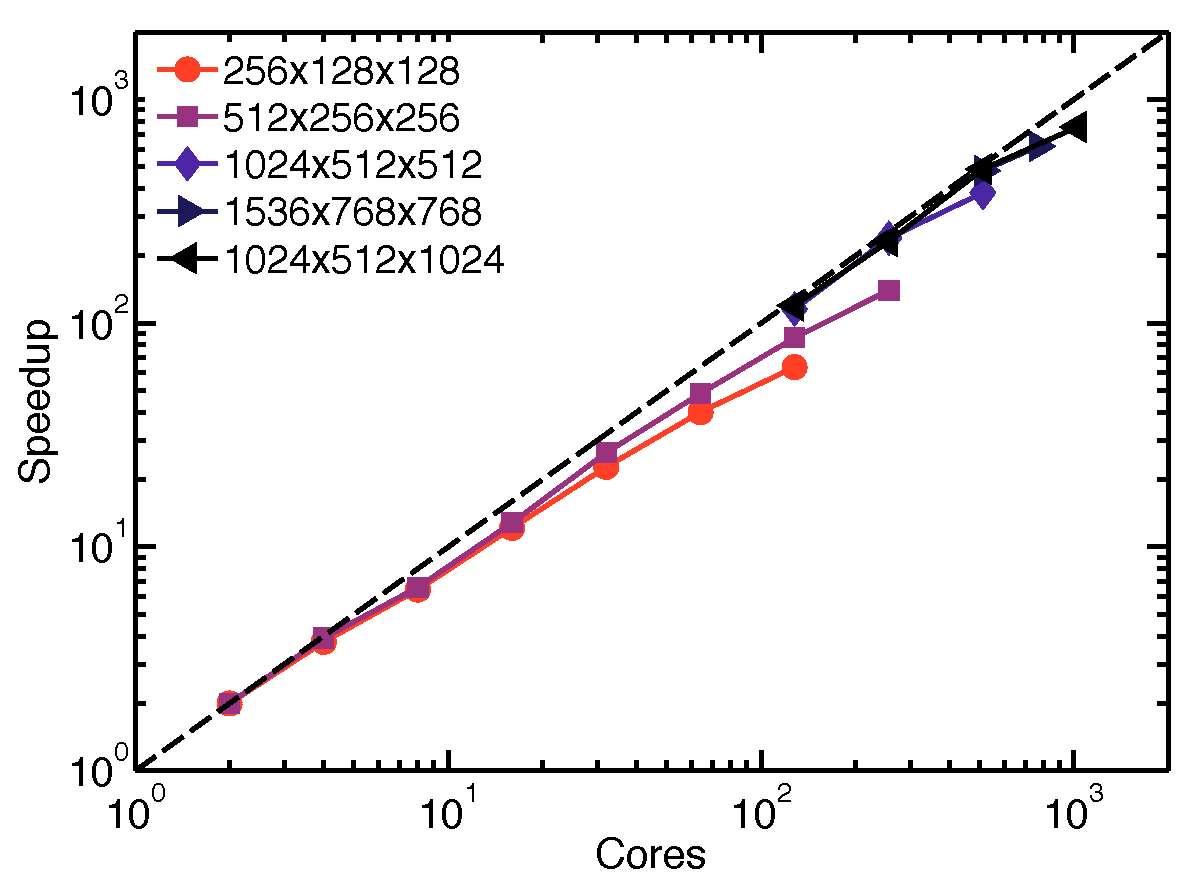
\includegraphics[width=0.85\textwidth]{scaling}
  \caption{Scaling of the code with the concurrent precursor method. The depicts speed up as a function of the number of computational cores.}
  \label{fig1}
\end{figure}

\printbibliography[heading=subbibliography,notkeyword=this]

\end{document}
